\documentclass[11pt, class=article, crop=false]{standalone}
\usepackage[subpreambles=true]{standalone}
\usepackage[T1]{fontenc} % for font setting
\usepackage{newtxtext,newtxmath}
\usepackage{import,
            graphicx,
            parskip,
            url,
            amsmath,
            wrapfig,
            fancyhdr,
            soul,
            tabularx,
            authblk,
            textcomp,
            lineno}

% side caption figure
\usepackage{sidecap}
\sidecaptionvpos{figure}{t}

% for special characters in bibliography            
\usepackage[utf8]{inputenc}
\usepackage[T1]{fontenc}

% citation setup
\usepackage[euler]{textgreek}
\usepackage[sort&compress]{natbib}
\setcitestyle{square}
\setcitestyle{comma}
\bibliographystyle{pnas-new}

% caption setup
\usepackage[font={f, small}, labelfont={bf, small}]{caption}
           
% color box
\usepackage[most]{tcolorbox}
\tcbuselibrary{breakable}

% margin
\usepackage[top=2.54cm, bottom=2.54cm, left=2.54cm, right=2.54cm]{geometry}%set margin

% title
\title{Geometric ecosystem complexity regulates food chains}
\date{} % remove date from title

% author list
\author[1]{Akira Terui}
\author[1,2]{Shota Shibasaki}
\author[3]{Justin P. F. Pomeranz}
\author[4]{Mason Ibrahim}
\author[1]{Ethan Isaac}
\author[1]{Ashley LaRoque}
\author[5]{Dai Yamazaki}
\author[6]{Jacques C. Finlay}
\affil[1]{Depatment of Biology, University of North Carolina at Greensboro}
\affil[2]{Center for Frontier Research, National Institute of Genetics}
\affil[3]{XXX, Colorado Mesa University}
\affil[4]{XXX, Duke University}
\affil[5]{Institute of Industrial Science, University of Tokyo}
\affil[6]{Departiment of Ecology, Evolution, and Behavior, University of Minnesota}

\linenumbers

\begin{document}

\maketitle

\section*{Abstract}
Since the time of Charles Elton, ecologists have been fascinated by the variation in food chain length among natural communities.
A prevailing view suggests that the size of an ecosystem is a key factor influencing food chain length (the ecosystem size hypothesis).
However, current discussions on FCL have lacked robust frameworks addressing the potential influence of spatial ecosystem complexity, a geometric characteristic independent of ecosystem size.
Here, we use theory and meta-analysis to demonstrate that ecosystem complexity, rather than ecosystem size, plays a crucial role in regulating food chains in rivers.
Our spatial theory suggests that the complex branching patterns of tributaries buffer downstream areas from cascading disturbances like floods, thereby allowing longer food chains to persist.
However, our theory predicts an ambiguous relationship between food chain length and ecosystem size (total river length of an entire watershed), a pattern that is substantially different from the prediction of the ecosystem size hypothesis.
A meta-analysis of global food chain data strongly supported these theoretical findings.
The complexity of river branching consistently had positive effects on riverine food chains worldwide, whereas the total river length showed no clear relationships.
This study provides a conceptual ground for understanding the organization of food webs in ecosystems with complex spatial structures.

% \section*{Significance}
% Why do food chain lengths -- the number of feeding links from producers to apex consumers in a food web -- vary in nature?
% This question has captivated ecologists since the early 20th century, and larger ecosystems were thought to support longer food chains.
% However, we found that the complexity of an ecosystem’s shape, such as the branching patterns of rivers, matters more than size.
% Intricate river branching can buffer downstream areas from disturbances like floods, allowing longer food chains to persist.
% We also observed an ambiguous relationship between food chain length and ecosystem size, challenging the idea that bigger is always better for food chains.
% This study highlights how the shape of ecosystems influences the organization of food webs.

\newpage

\section{Introduction}
Since Charles Elton coined the term ``food cycles'' in 1927 \citep{elton_animal_1927}, food webs have been a central theme in ecology \citep{paine_food_1966, pimm_food_1991, post_long_2002}.
In particular, the vertical structure of food webs, often measured as food chain length (FCL), has intrigued ecologists due to its implications for trophic dynamics, nutrient cycling, and biomagnification of environmental contaminants \citep{post_long_2002}.

In theory, FCL should increase with increasing ecosystem size \citep{schoener_food_1989}, resource availability \citep{oksanen_exploitation_1981}, and environmental stability \citep{pimm_number_1977} through the enhanced persistence of species populations.
Ample empirical evidence suggests that ecosystem size increases FCL in simple model ecosystems (e.g., oceanic islands) \citep{vander_zanden_patterns_1999, post_ecosystem_2000, takimoto_ecosystem_2008, doi_resource_2009} with multiple mechanisms proposed to explain the positive relationship \citep{takimoto_effects_2012, ward_mechanistic_2017, mcintosh_capacity_2018, terui_spatial_2019}.
Yet, mixed results are reported for resource availability and environmental stability hypotheses \citep{takimoto_environmental_2013, warfe_productivity_2013, guo_towards_2023}, partially due to complex interactions between internal food web structure and environmental drivers \citep{takimoto_effects_2012, shibasaki_food_2024}.
Although underlying mechanisms remain elusive, these findings have led to the prevailing view that factors associated with ecosystem size are a primary regulator of food chains.

Current frameworks, however, lack the ability to illuminate the role of geometric ecosystem complexity (``ecosystem complexity'') in regulating FCL.
Many natural systems display convoluted structures, characterized by repeating geometric patterns across spatial scales \citep{rodriguez-iturbe_fractal_2001, turner_landscape_2015}.
For example, dendritic ecosystems, such as trees and rivers, exhibit deep self-similarity in branching patterns, a hallmark of fractals \citep{rodriguez-iturbe_fractal_2001, terui_revisiting_2024}.
The prevalence of branching shapes habitat heterogeneity and spatial connectivity, underpinning the emergent stability of metapopulation dynamics \citep{yeakel_synchronisation_2014, moore_emergent_2015, terui_metapopulation_2018} and the spatial coexistence of competing species  \citep{terui_emergent_2021}.
Such influences of ecosystem complexity should ``pile up'' in a food web through predator-prey interactions.
Yet, previous studies on food webs predominantly assumed simplified landscapes for tractability, leaving this important question unanswered.

Here, we use mathematical theory to gain mechanistic insights into how ecosystem complexity controls FCL in rivers.
A key element in our model is the representation of landscape-scale disturbance cascades, a phenomenon ubiquitous in rivers \citep{swanson_flood_1998, nakamura_disturbance_2000, sarremejane_drought_2021} and other ecosystems \citep{connell_30year_1997, cansler_climate_2014}.
Our spatial theory predicts that the intricate branching of tributaries reduces the downstream propagation of cascading disturbance (e.g., floods, drying).
This mechanism promotes the persistence of long food chains within the landscape under common structural properties of river networks.
However, the relationship between FCL and ecosystem size is predicted to be indeterminate in the presence of spatial disturbance cascades.
Our theoretical predictions are supported by the results of a meta-analysis of global FCL data, which provides strong empirical evidence.
This study offers an important conceptual basis for understanding how food webs are organized in spatially complex ecosystems.

\section{Results and Discussion}

\subsection{Theoretical Prediction}

We consider a bifurcating branching ecosystem of total river length $L$ (ecosystem size) and branching rate $\lambda_b$ (ecosystem complexity).
Habitat patches are distributed randomly with density $h$ [river length$^{-1}$] along the river, resulting in the total number of habitat patches $N = Lh$.
In our framework, the branching rate $\lambda_b$ can be viewed as the average number of links per unit river length, where an individual link (or ``branch'') refers to a river segment (Figure \ref{fig:scheme}A).
Due to the bifurcating nature, the number of links $B$ in a network must be odd (Figure \ref{fig:scheme}A).
On average, ecosystems with higher branching rates encompass more confluences (see \textbf{Methods} for specific assumptions).

\begin{figure}
    \centering
    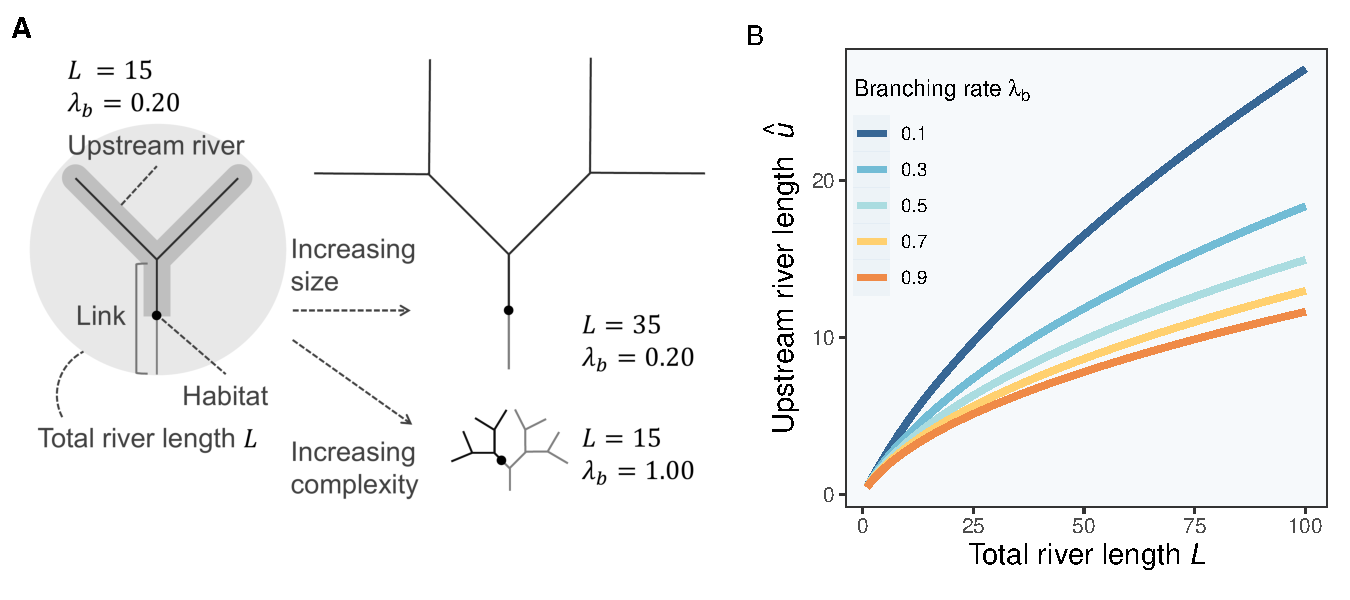
\includegraphics[width=\textwidth]{data_fmt/fig_theo_scheme.pdf}
    \caption{Modeling scheme. (A) Schematic representation of modeled branching networks. Each link represents a river segment, with confluences indicating where segments meet. Habitat patches (black dots) are randomly distributed along the network. The upstream river length $u$ (black solid lines) refers to the portion of the river located upstream from a given habitat patch (the expected value is on the Y-axis in panel B). As ecosystem size increases, the total river length ($L$) expands without affecting the branching rate ($\lambda_b$). In contrast, increasing ecosystem complexity raises the branching rate while keeping the total river length constant. (B) The upstream river length $u$ has the expected value $\hat{u}(L, \lambda_b)$, which is a nonlinear function of total river length $L$ and branching rate $\lambda_b$ (see Methods and \textit{SI Appendix}).}
    \label{fig:scheme}
\end{figure}

We model the patch occupancy dynamics of multi-trophic communities within the branching river network.
Let $p_k$ denote the proportion of habitat patches occupied for species $k$.
We describe the patch occupancy dynamics as:

\begin{equation}
    \frac{dp_k}{dt} = \gamma_{k} p_k (1 - p_k) - \mu_k p_k,
    \label{eq:model0}
\end{equation}

where $\gamma_k$ and $\mu_k$ denote colonization and extinction rates, respectively.
Here, we establish a connection between these parameters and spatial ecosystem properties, i.e., ecosystem size $L$ and complexity $\lambda_b$, as follows.

The colonization rate $\gamma_k$ is the number of effective propagules $c_{0,k}$ that successfully colonize habitat patches with establishment probability $r_k$ ($\gamma_k = c_{0,k} r_k$).
Propagules that survive the dispersal phase are referred to as ``effective.'' Thus, $c_{0,k}$ is a product of the gross number of propagules $g_k$ and survival probability during dispersal $\phi_k$.
However, we impose a habitat constraint on $c_{0,k}$ to realize $N$ is the possible maximum that effective propagules can colonize \citep{takimoto_effects_2012, terui_spatial_2019}:

\begin{equation}
    c_{0, k} = 
    \begin{cases}
        g_k \phi_k & \text{if $g_k \phi_k < N$},\\
        N & \text{if $g_k \phi_k \ge N$}.
    \end{cases}
    \label{eq:c0-prod}
\end{equation}

Given the relationship $N = Lh$, the colonization rate increases with increasing ecosystem size unless being limited by the species' ability to produce effective propagules.
We assumed that the establishment probability is proportional to resource supply $r_0$ for producers or the number of consumable prey for consumers (Methods).

The extinction rate comprises three potential sources of extinction, that is, disturbance, prey scarcity, and predation:

\begin{equation}
    \mu_{k} = 
        \underbrace{\mu_{k}^{(0)} (1 + \rho \hat{u})}_{\text{Disturbance}} + 
        \underbrace{\mu_{k}^{(1)} \left(1 - \frac{1}{|A_{k}|}\sum_{q\in A_{k}} p_{q} \right)}_{\text{Prey scarcity}} + 
        \underbrace{\mu_{k}^{(2)} \sum_{q \in \tilde{A}_{k}} p_{q}}_{\text{Predation}},
    \label{eq:extn-main}    
\end{equation}

where $\mu_k^{(0)}$, $\mu_k^{(1)}$, and $\mu_k^{(2)}$ are base parameters scaling the impacts of disturbance, prey scarcity, and predation, $\rho$ is the spatial synchrony probability, $\hat{u}$ is the expected upstream river length at a given habitat patch within a branching network, $A_{k}$ ($\tilde{A}_{k}$) is the set of consumable prey (predators) for species $k$, and $|A_{k}|$ is the number of consumable prey for species $k$.
For simplicity, we assumed constant values across species for $\mu_k^{(0)} = \mu^{(0)}$, and $\mu_k^{(2)} = \mu^{(2)}$.
Similarly, the prey effect $\mu_k^{(1)}$ was assumed to be zero for all producers and constant for all consumers ($\mu_k^{(1)} = \mu^{(1)}$).

The first term of Equation \ref{eq:extn-main} captures the downstream disturbance cascade.
In rivers, any disturbance event occurring upstream can propagate downstream through water movement, such as the spread of environmental contaminants \citep{massoudieh_biogeochemical_2010}, floods \citep{swanson_flood_1998, nakamura_disturbance_2000}, and droughts \citep{sarremejane_drought_2021}.
This propagation can lead to synchronized extirpation among flow-connected sites with a certain probability \citep{larsen_geography_2021, sarremejane_drought_2021}, denoted as the synchrony probability $\rho$. 
We assumed that such a risk of disturbance cascade is proportional to the upstream river length $u$, whose expected value $\hat{u}$ is a nonlinear function of total river length $L$ and branching rate $\lambda_b$ (Figure \ref{fig:scheme}B; Methods).
Therefore, the extinction dynamics are also linked to the spatial ecosystem properties.

\begin{table}[ht]
\centering
\caption{Parameter descriptions and values (analytical).\label{tab:parms}} 
\begingroup\small
\begin{tabularx}{\textwidth}{lll}
  \hline
Symbol & Description & Value (analytical) \\ 
  \hline
$r_0$ & Resource supply [-] & 0.40, 0.80 \\ 
  $g_0$ & Propagule size for producers [-] & 150 \\ 
  $\delta_0$ & Dispersal capability for producers [per unit river distance] & 0.50 \\ 
  $h$ & Habitat density [per unit river distance] & 2.50 \\ 
  $\mu^{(0)}$ & Disturbance rate [per unit time] & 2.50, 5.00 \\ 
  $\mu^{(1)}$ & Maximum prey-induced extinction rate [per unit time] & 5.00 \\ 
  $\mu^{(2)}$ & Predator-induced extinction rate [per unit time] & 0.00 \\ 
  $\rho$ & Synchrony probability [-] & 0.50 \\ 
  $\psi$ & Scaling exponent for propagule and dispersal parameters [per unit trophic position] & 0.50 \\ 
  $\theta$ & Degree of omnivory [per unit trophic position] & 0.25 \\ 
   \hline
\end{tabularx}
\endgroup
\end{table}


Using 20 replicas of realistic food webs (Methods), we evaluated how food chains respond to total river length $L$ and branching rate $\lambda_b$ across different levels of resource supply ($r_0$) and disturbance regimes ($\mu^{(0)}$).
These simulated food webs comprise 32 trophic species and vary in the number of trophic links and producers, allowing us to account for potential variations in food web structure.
In the absence of predation effects ($\mu^{(2)} = 0$), the unique FCL at stable equilibrium can be determined analytically by recursively solving Equation \ref{eq:model0} for $p_k$ from the base to the apex of the food web (Methods and \textit{SI Appendix}).

Ecosystem complexity (branching rate) was predicted to increase FCL regardless of ecological scenarios (Figure \ref{fig:sim-main}A and B).
Although resource supply and disturbance regimes influenced FCL, these factors did not alter the overall qualitative relationships (Figure \ref{fig:sim-main}).
A simple geometric mechanism underlies the consistency.
Branching divides the river network into flow-unconnected sub-networks, thereby dispersing the risk of synchronized extirpation due to flow-mediated disturbances.
Mathematically, this effect is manifested as a reduction in upstream river length $\hat{u}$ in complex, highly branched networks compared to simpler, less branched ones of similar sizes (Figure \ref{fig:scheme}B).
It is important to clarify that the positive effect of ecosystem complexity is contingent on the presence of spatial disturbance cascades; therefore, it disappears when omitting the impact of synchronized extirpation (Figures \ref{fig:sim-main}B and S1).

However, the predicted relationship between FCL and total river length ($L$) is either hump-shaped or vague, differing substantially from the prediction of the ecosystem size hypothesis (Figures \ref{fig:sim-main}A and \ref{fig:sim-main}C).
In our framework, we assumed that the probability of a disturbance cascade increases with increasing upstream river length $\hat{u}$, a monotonic increasing function of total river length $L$ (Figure \ref{fig:scheme}B) -- that is, the broader spatial coverage increases the likelihood that an episodic disturbance will occur in some part of the upstream flow-connected area.
Consequently, the greater frequency of synchronized extirpation can offset, or even exceed, the benefit of increased propagule sources in larger ecosystems.
Removing the effect of disturbance cascades therefore reverts the model prediction. 
In the absence of spatial disturbance cascades, the model predicted the positive influence of ecosystem size on FCL (Figures \ref{fig:sim-main}C and S1), a pattern consistent with previous food chain theory \citep{holt_food_2002, takimoto_effects_2012, terui_spatial_2019, guo_towards_2023}.


The analytical predictions remain robust even when relaxing the assumption to include predation effect ($\mu^{(2)} > 0$) and allowing variation in other ecological parameters, such as prey effect ($\mu^{(1)}$), propagule size ($g$), and trophic omnivory ($\theta$).
The positive relationship between FCL and branching rate was consistent, whereas the influence of ecosystem size on FCL was highly context-dependent (\textit{SI Appendix}).
An exception occurred only when high propagule production of producers ($g_0 = 150$) coincided with weak disturbance cascades ($\rho = 0.25$ and $\mu^{(0)} = 2.5$).
In these cases, nearly all species persisted regardless of ecosystem size and complexity, producing little variation in FCL.

\begin{figure}
    \centering
    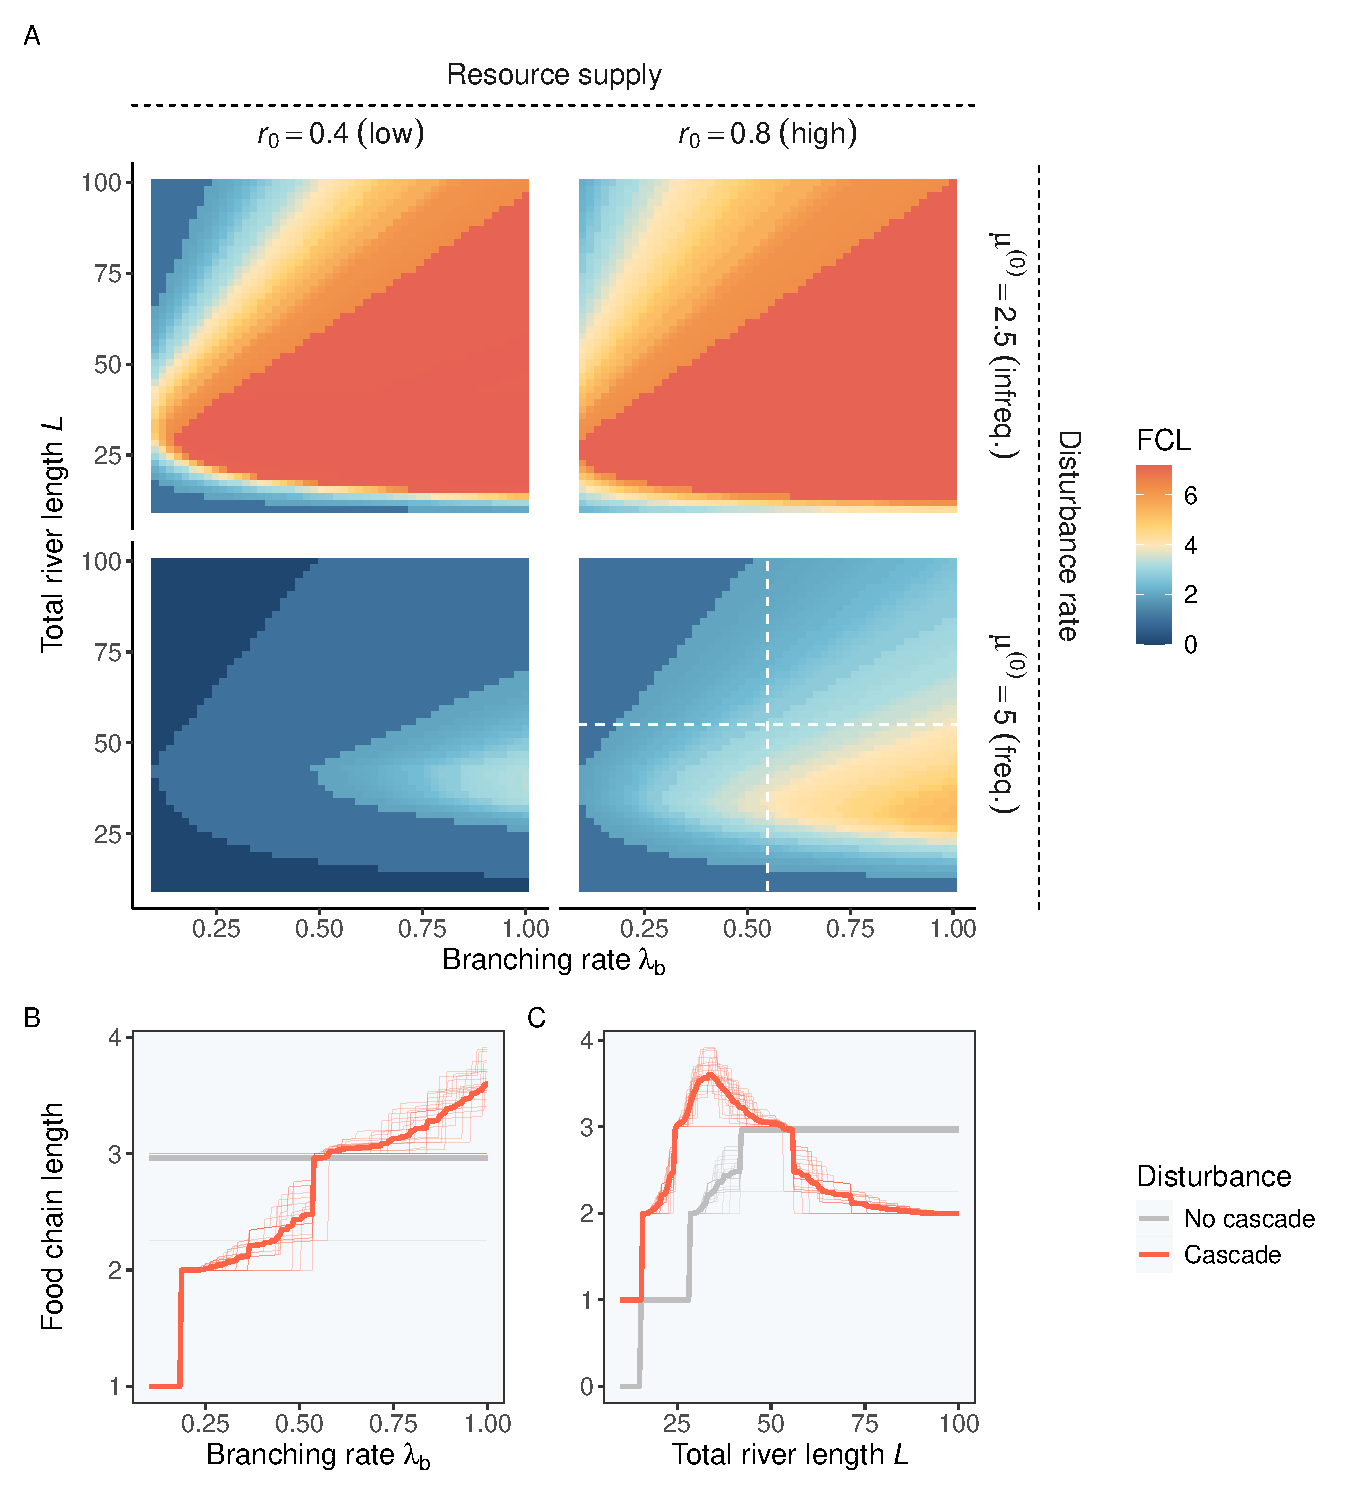
\includegraphics[width=0.8\textwidth]{data_fmt/fig_theo_main.pdf}
    \caption{Theoretical predictions of food chain length (FCL) based on ecosystem size and complexity. (A) Heatmap of FCL as a function of ecosystem size (total river length, $L$) and complexity (branching rate, $\lambda_b$), with rows and columns reflecting different disturbance and resource supply regimes. Each cell represents the average FCL of 20 food webs. White dashed lines indicate specific scenarios, explored in panels B (horizontal) and C (vertical). Additional parameter values are provided in Table \ref{tab:parms}. (B, C) Ecosystem complexity, but not size, significantly increases FCL in the presence of spatial disturbance cascades (red lines). The thick lines represent the average FCL of 20 food webs, while the thin lines depict individual food web predictions. When spatial disturbance cascades are removed, the positive effect of ecosystem complexity disappears (gray lines in panel B), yielding patterns consistent with the ecosystem size hypothesis (gray lines in panel C).}
    \label{fig:sim-main}
\end{figure}

\subsection{Empirical Evidence}

We empirically validate our theoretical predictions using stable isotope data on $\delta^{15}N$ from existing literature.
Our meta-analysis distinguishes itself from similar previous studies in its extent, extracting FCL estimates at 317 sites across 115 watersheds worldwide (Figure \ref{fig:fcl-obs}A).
To facilitate comparison with our theoretical predictions, ecosystem size and complexity were measured at the watershed level, where the total river length and the branching rate represent the properties of an entire watershed within which sampling sites are located (Methods).
These watersheds are separated by the ocean or lentic water bodies (e.g., lake), posing challenges to traverse across watersheds for lotic species (see Methods for watershed definition).
However, they are small enough (26 to $\sim$5,000 km$^2$) to assume that top predators can disperse therein at a multi-generation time scale \citep{comte_fish_2018}.
We employed Bayesian hierarchical modeling to evaluate the effects of ecosystem size (total river length [km]) and complexity (branching rate [km$^{-1}$]) on FCL.
We also accounted for potential influences of resource supply and disturbance through relevant proxy variables (Methods).

The results indicate that ecosystem complexity, rather than ecosystem size, is a key driver of increased FCL.
The analysis provided strong statistical support for the positive effect of branching rate (Figure \ref{fig:fcl-obs}B), with a high probability that the regression coefficient is positive ($\Pr(\beta > 0) = 0.95$; Figure \ref{fig:ridge} and Table S3).
Conversely, the effect of total river length was ambiguous (Figure \ref{fig:fcl-obs}C), characterized by the posterior distribution of its coefficient centered around zero (Figure \ref{fig:ridge}).
Interestingly, despite regional uniqueness in ecological communities and distinct evolutionary histories, a model comparison suggests that the regression coefficients for these ecosystem properties were constant among geographic regions.
That is, the model assuming constant slopes across geographic regions had the lower WAIC \citep{watanabe_asymptotic_2010} than the region-specific slope model ($-251.4$ vs. $-250.4$; see \textit{SI Appendix} for the competing model).
This result suggests the generality of our findings. 

\begin{figure}
    \centering
    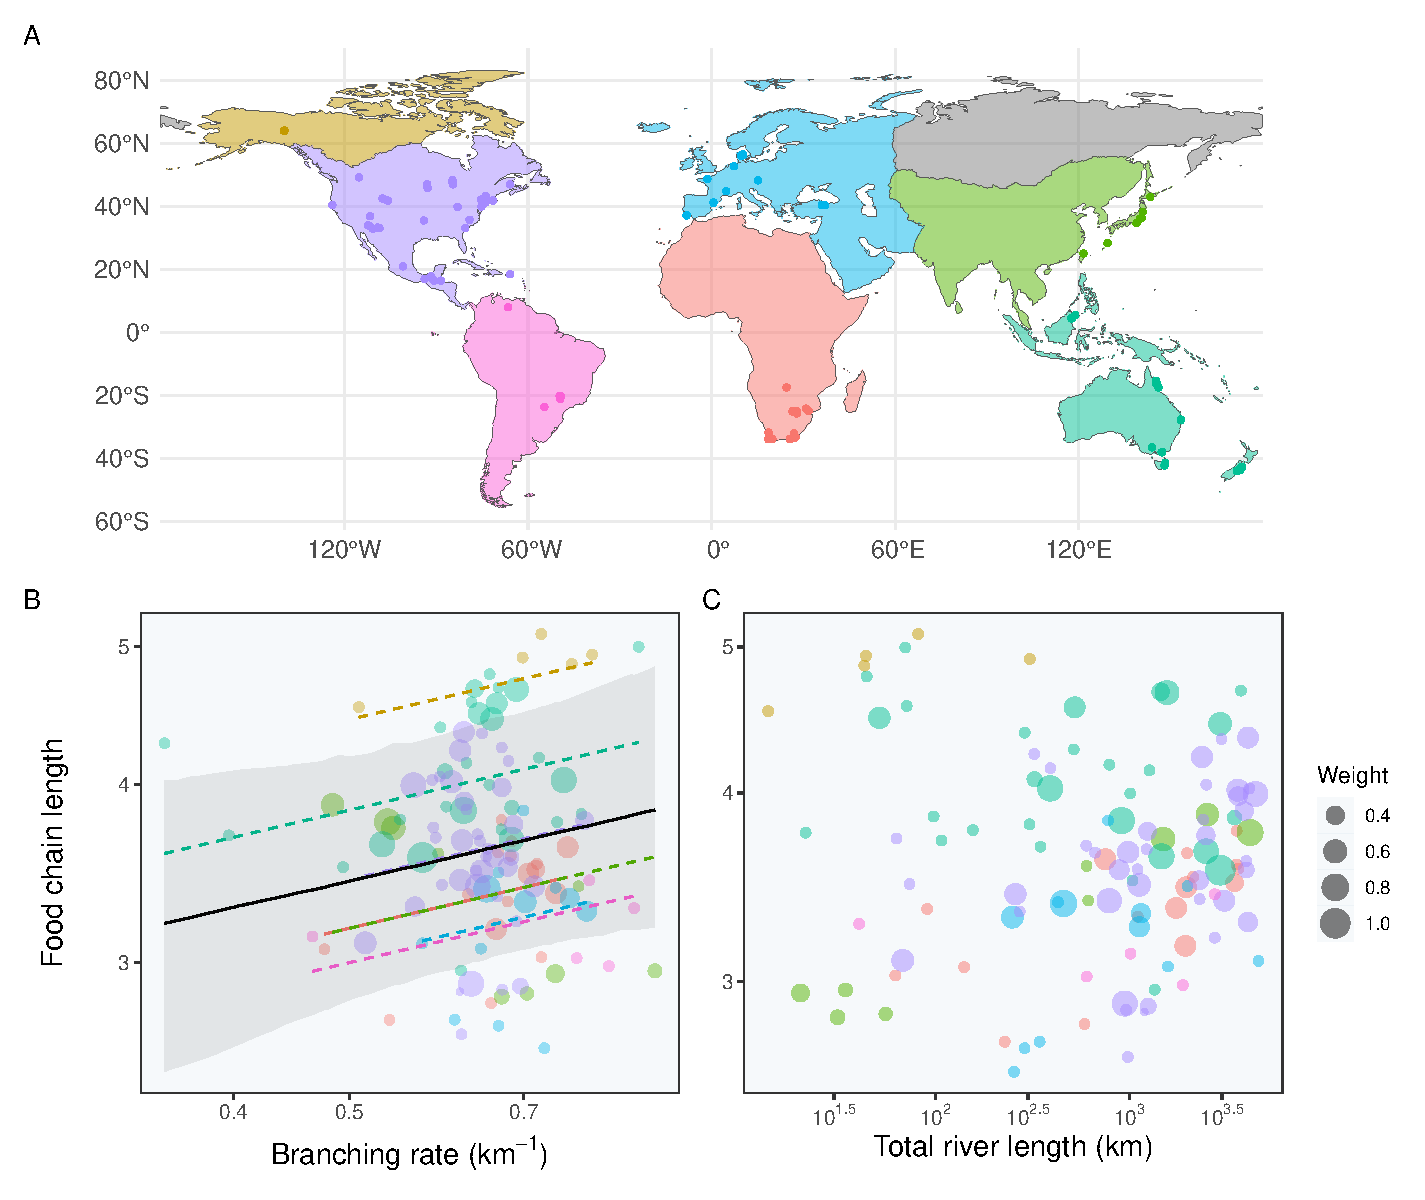
\includegraphics[width=0.9\linewidth]{data_fmt/fig_emp_fcl.pdf}
    \caption{Empirical regression analysis of food chain length (FCL) reveals the influence of ecosystem complexity. (A) Global map of sampling locations, with points representing outlet coordinates of 115 study watersheds. Colors indicate geographic regions categorized by HydroBASINS (level one) \citep{lehner_global_2013}. (B, C) Weighted robust regression. Circles show FCL estimates averaged for each watershed (i.e., parameter $\alpha_{0,w}$ in Equation \ref{eq:watershed-avarage}), and greater weights (proportional to circle size) were given to watersheds with more sampling sites and spatially random sampling (see Methods for details). Colors in the regression plots match the geographic region colors in panel A. The solid line represents the global model prediction with its 95\% credible interval (gray shade), while dashed lines show region-specific predictions (note: no regression lines in panel C due to weak statistical evidence). Note that the branching rate and the total river length represent the value of an entire watershed within which sampling sites are located.}
    \label{fig:fcl-obs}
\end{figure}

Our theory predicts that ecosystem complexity regulates FCL by dispersing the risk of disturbance cascades.
This buffering mechanism may explain the observed effect of branching because the wealth of observations suggests the prevalence of disturbance cascades in rivers \citep{swanson_flood_1998, nakamura_disturbance_2000, berghuijs_growing_2019, sarremejane_drought_2021, sharma_spatial_2024}.
For instance, in the Blue River watershed in the northwestern United States, half a century of records show that a significant proportion of debris flows travel over long distances, originating from confined mountain streams and cascading into larger downstream rivers \citep{nakamura_disturbance_2000}.
Recent studies unveiled an expanding range of spatial flood synchrony \citep{berghuijs_growing_2019, sharma_spatial_2024}, suggesting that the disturbance cascade perspective will become even more crucial under climate change.
Such hydrological processes are linked to the common occurrence of synchronized population dynamics \citep{sarremejane_drought_2021, larsen_geography_2021}.
An exemplary work by Larsen et al. \citep{larsen_geography_2021} demonstrated that fish population dynamics in flow-connected sites are highly synchronized, based on an analysis of over 34,000 pairs of fish population time series across Europe.

It is therefore reasonable that our data support the strong impact of precipitation on FCL (Figure \ref{fig:ridge}), which serves as a watershed-level proxy for disturbance regimes.
Our independent analysis of river discharge and precipitation suggested that extreme flow anomalies are more likely to occur in areas with higher precipitation (\textit{SI Appendix}).
Such anomalies, whether in the form of high or low flow, can increase the likelihood of species extirpation.
In parallel, high flow variability can reduce energy transfer efficiency within a food web, leading to shorter FCL \citep{baruch_food_2023}.
These processes may act in concert to constrain FCL in rivers with high precipitation.

The lack of ecosystem size effects is consistent with our theoretical predictions.
In contrast, several empirical studies have reported that ecosystem size can regulate riverine food chains \citep{mchugh_dual_2010, sabo_role_2010, mcintosh_capacity_2018}.
Our findings contradict these observations.
They, however, consider the effect of ecosystem size within an explicitly local context.
For example, McHugh et al. \citep{mchugh_dual_2010} used local stream size (e.g., the cross-sectional area of the study reach) as a metric of ecosystem size (hereafter, ``habitat'' size).
At this spatial scale, theory predicts that FCL should increase with increasing habitat size \textit{via} frequent colonization to larger habitats (i.e., target effects) \citep{shibasaki_food_2024}, metabolic scaling \citep{mcintosh_capacity_2018}, or weakened omnivory \citep{ward_mechanistic_2017}.
The site-level predictor of our hierarchical model captured some of these local effects of habitat size (see Methods) because FCL was longer in low-elevation streams with wide and open channels (Figure \ref{fig:ridge}).
The total river length quantifies the size influences at a broader landscape scale (i.e., watershed level), where statistical averaging may attenuate local variations. 
Thus, the present study speaks to the importance of spatial scale when examining the effect of ecosystem size on FCL.

Our analysis unveiled a negative influence of elevation on FCL (Figure \ref{fig:ridge}), and this pattern may reflect an elevational gradient of stream productivity \citep{marzolf_ecosystem_2021}.
Elevation may control gross primary production through diverse pathways, including light availability, water temperature, and nutrient availability \citep{marzolf_ecosystem_2021, atkinson_determinants_2018}.
In our dataset, high-elevation streams are characterized by small stream sizes (Methods), restricting light transmission to the water surface by shading \citep{finlay_light-mediated_2011, finlay_human_2013, bernhardt_light_2022}.
Additionally, lower water temperatures and nutrient availability in high elevations may limit stream productivity \citep{demars_temperature_2011}.
Although we could not yield direct measures of stream productivity at FCL sites, the negative influence of elevation provides indirect support for the resource availability hypothesis in rivers.


% Our analysis is dedicated to addressing the inherent heterogeneity in the dataset.
% First, we used environmental variables from consistent data sources through extensive geospatial analysis.
% Recent advancements in remote sensing, climate, and hydrological modeling empowered us to derive high-resolution environmental variables from publicly available geospatial layers.
% By leveraging these cutting-edge tools, we performed rigorous statistical inferences. 
Our advanced statistical modeling accounted for common challenges in meta-analysis, such as data outliers, unequal and non-random sampling efforts, and the imperfect sampling of stable isotope data (see Methods for details).
These quantitative techniques are crucial for our analysis, as they accommodate the variability in sampling schemes found in previous studies.
However, as with any empirical research, our findings should be interpreted with caveat.
We cannot rule out the possibility of spurious correlations, and experimental manipulations are warranted to confirm biological causality.
Although watershed-scale experiments are practically impossible, small-scale experiments of micro-organisms may provide an alternative means to test the causality \citep{altermatt_big_2015, green_long_2023}.

\begin{figure}
    \centering
    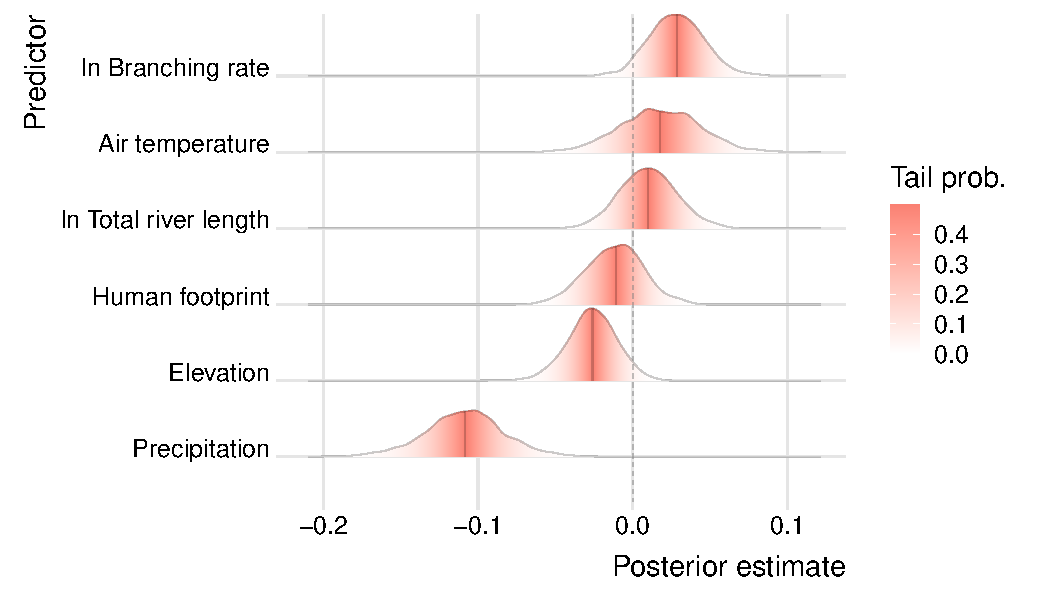
\includegraphics[width=0.75\linewidth]{data_fmt/fig_emp_ridge.pdf}
    \caption{Posterior distributions for the standardized regression coefficients. The Y-axis represents predictor variables, and colors are proportional to tail probabilities. Vertical lines are median estimates.}
    \label{fig:ridge}
\end{figure}

\subsection{Implications}
Over the past decades, discussions in FCL research have revolved around three major hypotheses: resource availability, environmental stability, and ecosystem size \citep{oksanen_exploitation_1981, pimm_number_1977, schoener_food_1989}.
However, little attention has been paid to ecosystem complexity despite the ubiquity of fractals across terrestrial \citep{turner_landscape_2015} and aquatic ecosystems \citep{rodriguez-iturbe_fractal_2001}.
Here, our synthesis provides the first evidence that ecosystem complexity regulates food chains in rivers, an exemplary case of spatially complex ecosystems.
The regulatory role of ecosystem complexity arises purely from the physical architecture of spatial network structure, likely explaining the remarkable consistency across geographic regions.
% Supporting this prediction, our meta-analysis demonstrates that ecosystem complexity controls FCL across diverse geographic regions, regardless of differences in species pools and evolutionary histories.
Although our focus is on river networks, there is no reason to believe that this concept is irrelevant to other ecosystems.
Forests exhibit complex vertical and horizontal structures, creating heterogeneous microhabitats with varying susceptibilities to wind and fire disturbances \citep{peterson_contagious_2002, cansler_climate_2014}.
Similarly, reef topography influences spatial disturbance patterns in marine systems \citep{connell_30year_1997}.
Therefore, the complexity should be seen as the rule, not the exception.

Climate change increases the frequency and magnitude of environmental disturbances, and ecosystem complexity may serve as a natural defense mechanism against these disruptive changes \citep{terui_metapopulation_2018, terui_emergent_2021, pomeranz_ecosystem_2023}.
However, human activities often simplify the spatial structure of ecosystems to manage production systems or mitigate natural disasters \citep{turner_landscape_2015, grill_mapping_2019, elmore_disappearing_2008}, likely eroding their inherent resilience to a changing climate.
% For instance, the complexity of river networks has been greatly reduced due to habitat fragmentation \citep{grill_mapping_2019} and stream burial \citep{elmore_disappearing_2008}.
Although conventional wisdom emphasizes the importance of ecosystem size, a radical shift in conservation principles may be necessary to foster resilient food webs in spatially complex ecosystems.

\newpage

\section{Methods}

\subsection{Theory}

\subsubsection{Food web construction}

We used the preferential prey model to generate initial food webs \citep{johnson_trophic_2014}.
We chose this method because it generates (i) food web structures comparable to those observed in nature and (ii) acyclic food webs \citep{shibasaki_food_2024}.
Although the niche model \citep{williams_simple_2000} is used widely in food web research, this algorithm is unsuitable for our study because it may create loops and cannibalism in a food web, which prevent us from defining trophic positions and FCL \citep{shibasaki_food_2024}.

The preferential prey model requires four parameters to build a food web: the number of (trophic) species $S$, the number of producer species $P$, the expected number of trophic links $N_l$, and trophic omnivory $\theta$ ($\theta > 0$).
In this model, a food web begins with $P$ primary producers, indexed as species $k = 1, 2, ..., P$.
Then, consumer species with index $k = P + 1, P + 2, ..., S$ are sequentially introduced and given their first prey $q$ randomly from those introduced earlier.
The parameter $N_l$ controls the number of additional prey, and consumer species $k$ choose, if any, additional prey $q'$ ($q' \ne q$) according to the trophic position of the first prey.
The probability of choosing prey $q'$, denoted as $Q_{q'}$, is proportional to trophic distance between $q$ and $q'$:

\begin{equation}
    Q_{q'} \propto e^{-\theta^{-1} |\tau_{q'} - \tau_q|},
\end{equation}

where $\tau_q$ is the structural trophic position of species $q$.
The trophic position of producers is one, and
consumer trophic positions are given as the average of prey trophic positions plus one:

\begin{equation}
    \tau_k = 
    \begin{cases}
    1 & ~\text{for producers}~ (k=1, 2, \ldots, P),\\
    1 + |A_{k}|^{-1} \sum_{q \in A_{k}} \tau_q & ~\text{for consumers}~ (k = P+1, P+2, \ldots, S),
    \end{cases}
    % \label{eq:def_tp}
\end{equation}

where $A_{k}$ and $|A_{k}|$ denote the set and the number of consumable prey for species $k$, respectively.
See \textit{SI Appendix} for further details.

\subsubsection{Spatial model}

We consider a bifurcating branching ecosystem of total river length $L$ and branching rate $\lambda_b$, in which $N$ habitat patches are distributed randomly with density $h$ [river length$^{-1}$] along the river (i.e., $N = Lh$).
In this system, the branching rate is a statistical parameter controlling the length of an individual ``link'' (Figure \ref{fig:scheme}A).
Specifically, the length of link $s$, denoted as $l_s$, is assumed to follow an exponential distribution as $l_s \sim \mbox{Exp}(\lambda_b)$ \citep{peckham_reformulation_1999, terui_metapopulation_2018, terui_emergent_2021}, but is conditional on $\sum_s^B l_s = L$ ($B$ denotes the number of links).
The average link length approaches $\lambda_b^{-1}$ as $\lambda_b L \rightarrow \infty$.

Here, we use the extension of the Levins metapopulation model to dictate the patch occupancy dynamics of interacting species within the branching river network \citep{calcagno_constraints_2011, takimoto_effects_2012, guo_towards_2023} (see \textit{SI Appendix} for derivation).
Let $p_k$ denote the proportion of habitat patches occupied for species $k$.
We describe the temporal dynamics as:

\begin{equation}
    \frac{dp_k}{dt} = \gamma_{k} p_k (1 - p_k) - \mu_k p_k,
\end{equation}

where $\gamma_k$ and $\mu_k$ denote colonization and extinction rates, respectively.
We express these parameters as functions of ecological processes and spatial ecosystem structure.

\textit{Colonization}. The colonization rate $\gamma_k$ is a product of establishment probability $r_k$ and the number of effective propagules $c_{0,k}$ ($\gamma_k = r_k c_{0,k}$).
We assumed that the establishment probability is proportional to resource supply for producers or prey availability for consumers:

\begin{equation}
    r_{k} = 
    \begin{cases}
        r_0 & ~\text{for producers}~ (k=1, 2, \ldots, P)\\
        |A_{k}|^{-1} \sum_{q~\in A_{k}} p_{q} & ~\text{for consumers}~ (k=P+1, P+2, \ldots, S)
    \end{cases}
\end{equation}

where $r_0$ ($0 \le r_0 \le 1$) is the resource supply, and $\sum_{q \in A_{k}} p_{q}$ ($q \ne k$) is the expected species richness of prey for consumer $k$.
Despite its simplicity, this formulation naturally accounts for the trade-off between specialist and generalist consumers because the impact of single prey species scales with the number of consumable species.

Effective propagule $c_{0,k}$ is a product of the gross number of propagules $g_k$ and survival probability during dispersal $\phi_k$.
We impose a habitat constraint on $c_{0,k}$ because $N$ is the maximum number of habitat patches that effective propagules can colonize \citep{takimoto_effects_2012, terui_spatial_2019}:

\begin{equation}
    c_{0, k} = 
    \begin{cases}
        g_k \phi_k & \text{if $g_k \phi_k < N$},\\
        N & \text{if $g_k \phi_k \ge N$}.
    \end{cases}
    \label{eq:c0-prod}
\end{equation}

The survival probability is described as $\phi_k = 1 - e^{-\delta_k h}$ so that dispersal capability $\delta_k$ and habitat density $h$ increase the survival during dispersal.
This assumption makes biological sense because habitat density decreases the mean distance between a pair of habitat patches \citep{terui_spatial_2019}.
We assumed that $g_k$ and $\delta_k$ scale with the species' structural trophic position $\tau_k$ as $\ln g_k = \ln g_0 - \psi \ln \tau_k$ and $\ln \delta_k = \ln \delta_0 + \psi \ln \tau_k$, where $g_0$ and $\delta_0$ represent the propagule and dispersal values for producers.
This assumption aligns with the known relationships of trophic position (or level) versus production \citep{finlay_stream_2011} and versus dispersal ability \citep{mccann_dynamics_2005}.

\textit{Extinction}. We express the extinction rate $\mu_k$ as a function of disturbance, prey scarcity, and predation:

\begin{equation}
    \mu_{k} = 
        \underbrace{\mu_{k}^{(0)} (1 + \rho \hat{u})}_{\text{Disturbance}} + 
        \underbrace{\mu_{k}^{(1)} \left(1 - \frac{1}{|A_{k}|}\sum_{q\in A_{k}} p_{q}\right)}_{\text{Prey scarcity}} + 
        \underbrace{\mu_{k}^{(2)} \sum_{q \in \tilde{A}_{k}} p_{q}}_{\text{Predation}},
    \label{eq:extn}    
\end{equation}

where $\tilde{A}_{k}$ is the set of predators for species $k$.
The disturbance term comprises two potential sources, $\mu^{(0)}_k$ and $\mu^{(0)}_k \rho \hat{u}$.
The first component $\mu^{(0)}_k$ is the stochastic disturbance occurring at the patch of interest.
The second component $\mu^{(0)}_k \rho \hat{u}$ is the influence of the downstream disturbance cascade, where $\rho$ and $\hat{u}$ denote the disturbance synchrony probability and the expected upstream river length at a given habitat patch, respectively.
% In rivers, any disturbance can cascade downstream as water flows downstream.
% For example, the impact of environmental pollutants may propagate downstream through water movement.
% Similarly, flood and drought disturbances are highly correlated between up- and downstream reaches, causing synchronized population dynamics of flow-connected sites.
The expected value $\hat{u}$ can be expressed as a nonlinear function of $L$ and $\lambda_b$ (see \textit{SI Appendix} for derivation):

\begin{equation}
    \hat{u}(L, \lambda_b) = L \sum_{z \in 2\mathbb{Z}_{\ge 0}} \left[ \frac{\hat{n}(z)}{z + 1} f'_{\text{pois}}(z; L, \lambda_b)\right] + \frac{1 - e^{-2 \lambda_b L}}{2 \lambda_b (1 + e^{-2 \lambda_b L})},
\end{equation}

where

\begin{equation}
    \hat{n}(z) = 2^{z + 1} \binom{z + 1}{\frac{z + 2}{2}}^{-1} - 2,
\end{equation}

and

\begin{equation}
    f'_{\text{pois}}(z; L, \lambda_b) = \frac{(\lambda_b L)^z e^{-\lambda_b L}}{z!} \cdot \frac{1 + (-1)^{z}}{1 + e^{-2\lambda_b L}}.
\end{equation}

The parameter $\rho$ independently controls the strength of up- and downstream synchronization.

In the second term of Equation \ref{eq:extn}, we assume that the extinction rate decreases with increasing species richness of available prey, and the parameter $\mu_{k}^{(1)}$ denotes the extinction rate in the complete absence of prey ($\mu_{k}^{(1)} = 0$ for producers).
Predation pressure is assumed to increase linearly with the species richness of predators $\sum_{q \in \tilde{A}_{k}} p_{q}$.
The parameter $\mu_{k}^{(2)}$ defines how quickly the predator-induced extinction rate increases with the predator richness.

In the absence of predator-induced extinction ($\mu_{k}^{(2)}=0$), the equilibrium of the system can be derived analytically.
According to  Equation \ref{eq:model0}, the fraction of patches occupied by species $k$ at equilibrium is written as follows:

\begin{equation}
    \frac{dp_k}{dt} = 0 \Leftrightarrow p_k = \left\{\begin{array}{c}
         0,\\
         p_{k}^{*}, 
    \end{array}
    \right.
\end{equation}

where $p_{k}^{*} = 1 - \mu_k / \gamma_k$. 
For producers ($k=1, 2, \ldots, P$), $\gamma_k$ and $\mu_k$ are constants.
The occupancy at equilibrium is therefore either persistent ($p_k = p_k^* > 0$) or extinct ($p_k = 0$).
For consumers ($k = P+1, P+2, \ldots, S$), the occupancies of species $q = 1, 2, \ldots, k - 1$ can affect $p_k$, but not $q = k + 1, \ldots, S$.
Although this implies many possible combinations of equilibrium states (i.e., binary permutations of persistent or extinct), we demonstrated that the system has a unique stable equilibrium (see \textit{SI Appendix}).
This results in a single ``realized'' FCL at stable equilibrium (Equation \ref{eq:def_tp}).

%We consider the feasible case where $p_{k}^{*} > 0$ for all $k=1, 2, \ldots, S$.This is a necessary and sufficient condition for the local stability of the feasible equilibrium (\textit{SI Appendix}).Next, we show that the feasible equilibrium is, if exists, unique. For producers ($k=1,2,\ldots, P$), $\mu_k$ and $\gamma_k$ are independent of $\Vec{p}=\left(p_1, p_2, \ldots, p_S\right)$. Thus, $\hat{p}_k$ is unique for all producers.For consumers ($k=P+1,P+2,\ldots, S$), $\mu_k$ and $\gamma_k$ \textit{depend} on $\Vec{p}$. Nevertheless, because we assume acyclic food webs, $\mu_k$ and $\gamma_k$ depend only on $\left(p_1,p_2, \ldots, p_P,\ldots, p_{k-1} \right)$. This allows us to obtain $\hat{p_k}$ recursively. For example, $\hat{p_{P+1}}$ is unique because $\left(p_1, p_2, \ldots, p_P\right)$ is unique. Then, $p_{P+2}$ is also unique. This calculation can be continued until $k=S$.

\subsubsection{Model analysis}

In our analytical exploration, we considered 20 replicas of food webs comprising 32 species ($S = 32$) with the omnivory level observed in the wild ($\theta = 0.25$) \cite{johnson_trophic_2014}.
These food webs are simulated with different parameter values, which are drawn randomly as $P \sim \mbox{Pois}(0.19 \times S)$ (the number of producers) and $N_l \sim \mbox{Pois}(0.11 \times S^2)$ (the expected number of trophic links).
The expected means of these parameters were determined to reflect the typical values for the proportion of producers ($P / S \approx 0.19$) \citep{briand_community_1984} and connectance in nature ($N_l / S^2 \approx 0.11$) \citep{dunne_food-web_2002}.
We crossed these 20 food webs with resource supply ($r_0 \in \{0.4, 0.8\}$) and disturbance levels ($\mu^{(0)} \in \{2.5, 5.0\}$) with other parameter values summarized in Table \ref{tab:parms}.
In each simulation scenario, we systematically varied total river length $L$ and branching rate $\lambda_b$ as $L \in [10, 100]$ and $\lambda_b \in [0.1, 1.0]$ (50 values with an equal interval) to assess their influences.
This analytical exploration results in $20 \times 2^2 \times 50^2 = 200,000$ runs.
Note that we explored a broader parameter space using numerical analysis in \textit{SI Appendix}.

At (quasi)equilibrium, we calculated the ``realized'' trophic position $\tau^{(w)}$ for persistent species as follows.
Producers are assigned $\tau^{(w)} = 1$.
Consumer's $\tau^{(w)}$ is calculated as the weighted average of the prey's trophic positions plus one:

\begin{equation}
    \tau^{(w)}_k = \frac{\sum_{q \in A_{k}} p_{q} \tau^{(w)}_q}{\sum_{q \in A_{k}} p_{q}} + 1
    \label{eq:def_tp}
\end{equation}

We report the maximum value of $\tau_k^{(w)}$ as the predicted FCL in a given environmental context.
The analysis was performed in R 4.3.2 \citep{r_program}.

\subsection{Meta-analysis}

\subsubsection{Stable isotope data}

We performed a meta-analysis of empirical studies to examine environmental drivers of food chain length in rivers.
We assembled stable isotope data on $\delta^{15} N$ (\textperthousand) or trophic position estimates from three sources.
First, we used a systematic search. 
Our search was conducted on January 28, 2021, with the search term ``("food chain length")AND (stream* OR watershed* OR river*) AND ("stable isotope*")'' in Scopus.
Second, we examined studies used in the previous meta-analysis by Vander Zanden and Fetzer \citep{vander_zanden_global_2007}.
Lastly, we included peer-reviewed articles identified as potentially relevant \textit{via} non-systematic reviews to encompass important research not captured by our systematic search.
Our review identified 122 studies as potential data sources.

We used the following inclusion criteria to choose sites with sufficient information for our statistical analysis.
Each site (i) must contain either stable isotope data of nitrogen ($\delta^{15}N$) for top and baseline species (primary producer or consumer) or an estimate of the maximum trophic position; 
(ii) must contain reliable spatial coordinates for geospatial analysis; 
(iii) must be located within a freshwater lotic system, excluding lentic (reservoirs, wetlands, lakes) and semi-lentic systems (large rivers with $>$ 5000 km$^2$ in watershed area); and (iv) can be associated with potential environmental drivers in GIS.

We also obtained information on whether stable isotope data at each site included the isotopic signature of a suitable top predator in the system.
We categorized the site as ``a suitable top predator collected'' if the study explicitly stated so or targeted the top consumer community (typically fish) for stable isotope analysis.
We used this information to properly account for the imperfect sampling of top predators in our statistical analysis.
After this screening process, we retained 317 sites located in 115 watersheds from 46 studies (\textit{SI Appendix}, Table S3). 

When $\delta^{15}N$ values are available, we used the following equation to estimate FCL:

\begin{equation}
    \mbox{FCL} = \frac{\delta^{15}N_{\text{top}} - \delta^{15}N_{\text{base}}}{\Delta_N} + \tau_{\text{base}},
    \label{eq:fcl-si}
\end{equation}

where $\delta^{15}N_{\text{top}}$ and $\delta^{15}N_{\text{base}}$ are the stable isotope values for the top and baseline species, respectively.
$\Delta_{N}$ denotes the trophic enrichment factor, while $\tau_{\text{base}}$ represents the trophic position of the baseline species (one for primary producers and two for primary consumers). 
In this study, we assumed a trophic enrichment factor of $\Delta_{N} = 3.4$ following Post \citep{post_using_2002}.
For any instances where FCL estimates were originally calculated using a different $\Delta_{N}$ value but raw $\delta^{15}N$ values are not available, we recalculated these estimates using $\Delta_{N} = 3.4$ to maintain consistency across comparisons.

\subsubsection{Environmental variables}

We assembled environmental data at site and watershed levels.
The site-level environment refers to the environmental value at the sampling site.
At this level, we obtained the following variables: upstream watershed area [km$^2$] and elevation [m].
We delineated watershed polygons with MERIT Hydro version 1.0.3 \citep{yamazaki_merit_2019} to estimate the upstream watershed area at each site.
We extracted the elevation from the MERIT DEM (3 arc-second) \citep{yamazaki_high-accuracy_2017}.

At the watershed level, we obtained the following variables: total river length [km], branching rate [km$^{-1}$], mean annual air temperature [$^\circ$C], annual precipitation amount [kg m$^{-2}$], and human footprint index [-].
In our analysis, watersheds were separated by either the ocean, large lakes/reservoirs (10 km$^{2}$ in area), or large rivers that represent semi-lentic habitats (5000 km$^{2}$ in watershed area), which were extracted from Global 3 arc-second Water Body Map version 1.3 \citep{yamazaki_development_2015} and MERIT Hydro version 1.0.3 \citep{yamazaki_merit_2019}.

For each watershed, we delineated the watershed polygon and river polylines ($>$ 1 km$^2$ in watershed area) with MERIT Hydro to estimate the total river length and branching rate.
The total river length is the summed length of river polylines.
We estimated the branching rate as the inverse of the mean link length (= distance from one confluence to another or the river terminal [upstream river origins or river mouth]).
The inverse of the mean link length is an empirical proxy for theoretical branching rate $\lambda_b$ because it corresponds to the maximum likelihood estimate of the rate parameter of an exponential distribution \citep{terui_revisiting_2024}.

We took the spatial average of air temperature, precipitation, and human footprint index for each watershed polygon, whose data were sourced from CHELSA BIOCLIM+ (average of 1981-2010, 30 arc-second) \citep{brun_global_2022} and a global Human Footprint dataset populated by Mu et al \citep{mu_global_2022}.
For the Human Footprint Index, we used data from 2000, 2005, ..., 2015 (5-year interval), and extracted values from the year nearest to the first sampling year in each watershed.
We used the following R packages for our GIS analysis: \textit{sf} \citep{pkg_sf}, \textit{terra} \citep{pkg_terra}, \textit{exactextractr} \citep{pkg_exactextractr}, \textit{whitebox} \citep{pkg_whitebox}, and \textit{stars} \citep{pkg_stars}.

\subsubsection{Statistical analysis}

We used a hierarchical linear model to assess the influences of environmental variables on FCL.
Our stable isotope data provides suitable estimates of FCL only when top predators are included.
Otherwise, the estimates are imperfect and represent only a possible minimum at the site (i.e., right censored).
We accounted for this imperfect sampling with censored regression \citep{terui_stream_2018, lunn_bugs_2012}.
Let $y_i$ denote the suitable estimate of FCL at site $i$ after log transformation.
Our observed FCL estimate $Y_i$ (log transformed) is linked to $y_i$ as:

\begin{equation}
    y_i 
    \begin{cases}
        = Y_i~\text{if a suitable top predator is included (observed)},\\
        > Y_i~\text{if a suitable top predator is not included (censored).}
    \end{cases}
\end{equation}

Writing $f(\cdot;\Theta)$ as the probability density of a specified model with parameter vector $\Theta$, each observed data point contributes $f(Y_i;\Theta)$ to the likelihood of $\Theta$ whereas a censored data point provides a contribution of $\Pr(y_i > Y_i~|~\Theta) = \int_{Y_i}^{\infty} f(y_i;\Theta) dy_i$.
With this formulation, the censored regression corrects for possible biases in statistical inference (e.g., coefficients) \citep{terui_stream_2018, lunn_bugs_2012}, allowing us to use the data from imperfect sampling.

Our model assumed that $y_i$ follows a Student's t distribution as $y_i \sim t(\mu_{y,i}, \sigma^2, \nu)$.
We chose a Student's t distribution as an error structure because uncontrollable data anomalies may exist due to the nature of meta-analysis.
A Student's t distribution is robust to outliers, thereby providing conservative estimates of regression parameters \citep{lunn_bugs_2012}.
The expected value $\mu_{y,i}$ is related to site-level linear predictor(s) as:

\begin{equation}
    \mu_{y,i} = \alpha_{0, w[i]} + \sum_m \alpha_m x_{m,i},
\end{equation}

where $\alpha_{0, w[i]}$ is the watershed specific intercept for watershed $w$ ($w[i]$ denotes site $i$ nested within watershed $w$), and $\alpha_m$ is the coefficient for the $m$-th site-level predictor $x_{m, i}$.
At this level, we considered the local elevation at the site. 
Elevation was used as a collective proxy for gross primary production (GPP) because: (i) in our data, it moderately but significantly correlated with the log-transformed upstream watershed area (Pearson's product-moment correlation $= -0.43$, $p < 0.001$), which controls light availability and GPP in streams \citep{finlay_light-mediated_2011, finlay_stream_2011, bernhardt_light_2022}; (ii) a meta-analysis showed an elevational gradient of GPP in streams and rivers \citep{marzolf_ecosystem_2021}.
We did not include the upstream watershed area to avoid over-control bias \citep{arif_predictive_2022}.

We related watershed-specific intercept $\alpha_{0, w}$ (the expected average FCL at watershed $w$) to watershed-level predictors as:

\begin{equation}
    \alpha_{0, w} = \beta_0 + \sum_m \beta_m x'_{m, w} + \eta_{u[w]} + \varepsilon_{w},
    \label{eq:watershed-avarage}
\end{equation}

where $\beta_0$ is the global intercept, $\beta_m$ the regression coefficient for the $m$-th watershed-level predictor $x'_{m, w}$, $\eta_{u[w]}$ the random effect accounting for geographic variations, with $u$ denoting the index for each geographic region defined by HydroBASINS level-1 (c.f. Lehner et al. \citep{lehner_global_2013}; see Figure \ref{fig:fcl-obs}A).
At this level, we considered ecosystem size (log-transformed total river length), ecosystem complexity (log-transformed branching rate), climatic conditions (mean annual air temperature and annual precipitation amount), and human influences (human footprint index).
The random effect $\eta_{u[w]}$ was assumed to follow a normal distribution as $\eta_{u} \sim \mbox{Normal}(0, \sigma_{\eta}^2)$.
While Equation \ref{eq:watershed-avarage} represents a random intercept model, we also developed a random intercept-slope model as an alternative model, in which the effects of ecosystem size and complexity vary by region (\textit{SI Appendix}).

The parameter $\varepsilon_w$ the watershed-level residual errors, and we scaled $\varepsilon_w$ to assign higher weights to watersheds (i) with more sampling sites and (ii) with spatially random sampling design:

\begin{align}
    \varepsilon_w &\sim \mbox{Normal}(0, \sigma_{\varepsilon}^2 \zeta_w^{-1}),\\
    \zeta_w &\propto N_{s, w}^{\xi_1} e^{-\xi_2 (1 - d_{w})^2},
\end{align}

where $\sigma_{\varepsilon}^2$ is the residual variance, and $\zeta_w$ is the weight for watershed $w$, which is assumed to be proportional to a product of the number of sampling sites $N_{s,w}$ and the randomness factor $\exp[-\xi_2 (1 - d_{w})^2]$.
The spatial randomness of sampling sites was assessed by distance ratio $d_{w}$.
The distance ratio compares the median distance of observed site pairs to that of replicated ``random'' site pairs simulated along the same river network (see \textit{SI Appendix} for details).
If spatially biased, the distance ratio shows deviation from one, where $d_{w} < 1$ and $d_{w} > 1$ indicate over-aggregation and over-dispersion, respectively.
The Gaussian function $\exp[-\xi_2 (1 - d_{w})^2]$ returns smaller values as $d_{w}$ deviates from one, thus awarding more weights if spatially random.
The parameters $\xi_1$ and $\xi_2$ control how quickly $\zeta_w$ increases with the number of sampling sites and the spatial randomness, and these were estimated through the stochastic search of Bayesian inference.

We fitted our model to the data using NIMBLE version 1.2.1 \citep{nimble, pkg_nimble} in R 4.3.2 \citep{r_program}.
We assigned weakly informative priors to parameters: $\alpha_m,~\beta_0,~\beta_m \sim \mbox{Normal}(0, 5^2)$; $\sigma,~\sigma_{\varepsilon},~\sigma_{\eta} \sim t^+(0, 1, 10)$; $\xi_1 \sim \mbox{Normal}^+(0, 1)$; $\xi_2 \sim \mbox{Normal}^+(0, (\ln 10)^2)$; and $\nu \sim \mbox{Trunc(Exp}(0.1); 2, \infty)$, where plus signs indicate half-Normal or half-t distributions. 
Four Markov chain Monte Carlo (MCMC) chains were run until parameter estimates
converged.
The total number of MCMC iterations per chain was 60,000, in which MCMC samples were saved every 60 steps after the initial 30,000 burn-in period.
As a result, we used a total of $500 \times 4 = 2,000$ MCMC samples for the estimation of posterior distributions.
Convergence was assessed by examining whether the R-hat indicator of each parameter approached < 1.1 \citep{gelman2013bayesian}.

\section{Data availability}

Data and codes used in this study are available at:
\url{https://github.com/aterui/public-proj_fcl-river-synthesis}.
Functions used for our theoretical analysis are available as R packages \texttt{mcbrnet} (preferential prey model) and \texttt{rpom} (spatial model).

\section{Conflicts of Interest}

None declared.

\section{Ethics}

No live animals were used in this study.

\section{Acknowledgements}

We extend our gratitude to Yutaka Osada and Ryosuke Iritani for their valuable contributions to Lemma 1.3.2, as well as to Aisha Hamoud and Lucia Ramirez-Joseph for their assistance with the meta-analysis.
Our meta-analysis would not have been possible without the previous studies listed in \textit{SI Appendix} and the generous provision of raw data from several authors of the published articles.
This material is based upon work supported by the National Science Foundation through the Division of Environmental Biology (DEB 2015634).

\bibliography{references, ref_package, ref_book}

\end{document}